\section{Background}
\label{sec:background}
\subsection{FPGAs in space}\label{subsubsec:fpga}
Initially, FPGAs implemented only auxiliary tasks and glue logic in a spacecraft system. The basic telemetry and flight control tasks are handled by specialized CPUs, which is the topic of subsection of \ref{subsubsec:cpu}. However, FPGAs have recently gained increased popularity for aerospace applications, due to the increased processing power and size, weight, power, and cost (SWAP-C), when compared to CPUs and GPUs \cite{Lentaris2018}. In addition,  While continuing to support these functions, FPGAs are widely used for embedded computing in Space. For example, in \cite{Tsigkanos2020}, a Hyperspectral Image Compression implementation for CCSDS 123.0-B1 recommended standard is introduced, which is built on a COTS SoC. FPGAs are the de-facto solution for demanding processing acceleration applications, like deep-learning algorithms in neural networs.\cite{Vidmar2021}.\par
There only a limited number of Radiation Hardened By Design (RHBD) FPGAs in the market. The most important device families are manufactured by Microsemi and Xilinx \cite{leon21}. A common feature of these families is that the configuration memory is SRAM, instead of flash, since the latter technology is susceptible to radiation effects \cite{Marinella21}, with an obvious impact on the cost. The products of both vendors share a rich mission heritage, an extensive overview of which is also provided in \cite{leon21}.\par
In addition to the standard hardening techniques, Microsemi PolarFire radiation tolerant FPGAs chips use Silicon-Oxide-Nitride-Silicon (SONOS) Non-Volatile (NV) technology \cite{sonos}, which provides immunity against SEU effects, in addition to low power. The physical layer manufacturing details of the SONOS technology, as well as its rad-hard attrbutes are widely covered in \cite{sonos}. TMR in the user logic, when required, is assured through suitable provisions from the bundled software (Libero sinplify).\par
On the other hand, the Xilinx SRAM radiation hardened FPGA range includes the legacy Virtex-4QV FPGA (90nm) device family, the Virtex-5QV FPGA (65nm) XQR5VFX130 device and the RT Kintex UltraScale (20 nm) XQRKU060 device, which is currently the state-of-the-art in terms of performance.\par
In both cases which offers a wide selection of RHBD FPGAs, which have a long heritage in space missions. With their vendors being based in the USA, however, all these products are subject to USA export controls, which adds insecurity to the European missions' planning. Recently, the NanoXplore family of RHBD devices has been introduced as a European solution, although it has not yet presence in space.\par
Interestingly, an emerging trend for extending the application area of commercial Xilinx ZynQ and ZynQ Ultrascale+ SoCs into aerospace applications has risen recently. A number of research activities has been focusing on the study of the susceptibility of the ZynQ-7000 series SoCs. The SEU behaviour of the ZynQ-7020 SoC's integrated ARM Processing System is the subject of the work in \cite{Hiemstra2015}. In \cite{Tambara15}, the authors present their results on heavy proton SEU testing of the same device, while \cite{Bezerra17} evaluates the SEE behaviour of the NINANO board used in EYE-SAT nanosatellite. The work in \cite{Vlagkoulis21} is the most complete analysis of the SEE behaviour of ZynQ-7000 series programmable logic and configuration memory under heavy ion irradiation. One of its major contributions is that it provides the tools for the design of efficient mitigation techniques, including effective ECC and configuration memory scrubbing. At the same time, a multitude of research activities incorporate these SoCs for aerospace applications. In \cite{Tsigkanos2020}, for example, we have introduced a high performance parallel implementation of an accelerator for the CCSDS 123.0-B-1 hyperspectral compression algorithm. This work leverages the resources of both the processing system and the programmable logic to deliver state-of-the-art throughput performance. The authors in \cite{Sabogal19} propose a hybrid convolutional neural network accelerator for semantic segmentation of image, which is widely used in space applications. Their work is evaluated on Xilinx ZynQ and ZynQ Ultrascale+ MPSoCs, while performing error injection and radiation-beam testing, in order to characterise the response of the proposed architectural framework in the presence of radiation phenomena. In all these cases, mostly soft techniques are used as mitigation measures. TMR effectiveness under heavy ion radiation is evaluated in \cite{Sanchez19} for a ZynQ 7000 SoC supporting a  CCSDS 121.090-B-2 compression IP core, demonstrating a 40\% increased Mean Time To Failure (MTTF). A rather complete study of the effectiveness of soft methods is presented in \cite{Kibar19}. The key takeaway is that for non mission critical systems, soft SEE mitigation techniques can provide the resilience required for space applications.\par
In DSCAL, the following boards are available and used in the scope of the current thesis:
\begin{itemize}
    \item The KCU105 evaluation board, built around the Kintex UltraScale XCKU040 device, which is the commercial equivalent of the radiation tolerant Kintex Ultrascale XQRKU060. Regarding the rest of the board's equipment, of notable interest are the two SFP+ cages, which were used for spacefibre integration and the 2 GB of DDR4 RAM memory.
    \item The ZC706 board, featuring a Zynq-7000 XC7Z045 SoC at speed grade 2, with two ARM Cortex-A9 MPCore hard processors. One SFP+ cage is also included. The board also includes 1 GB of DDR3 RAM connected to the processing system (PS) build around the two ARM processors (component memory), as well as 1 GB of DDR3 RAM for the programmable logic (SODIMM memory). Access to the two memories is independent (both memories can be accessed at the same time).
    \item The Zedboard, with the Zynq-7000 SoC XC7Z020. The board has no SFP+ connections, but it includes 512MB DDR3 memory connected to the processing system. Access to the memory space from the programmable logic can be provided from the ZynQ's PS AXI3 high performance (HP) ports, as detailed in Section 
\end{itemize}

\subsection{Space-grade CPUs}\label{subsubsec:cpu}
Similarly to what is described in Section \ref{subsubsec:fpga}, the requirements of CPUs are radically different between terrestrial and aerospace applications. Commercial CPUs, target hugely larger market shares, can meet lower time to market requirements and include advanced features and vastly higher performance. Not being able to withstand the harsh environmental conditions typically met in spaceflight, however, they fail to meet the reliability requirements of space missions. Space-qualified CPUs have therefore been developed to mitigate these issues. These CPUs are based on commercial Instruction Set Architectures (ISAs), so the cost of the ecosystem around them is reduced. The ecosystems includes hardware design processes and tools, as well as software tools for applications development. Historically, MIL-STD-1750 architecture \cite{MIL-STD-1750} dominated space missions, due to its already widespread adoption by military airborne computers. Quickly, however, following the evolution of commercial architectures, the market was dominated by SPARC and PowerPC. A pictorial overview of the historical evolution of space CPUs is provided in Fig.\ref{fig:CPU-Archs}. 
	\begin{figure}
		\centering
		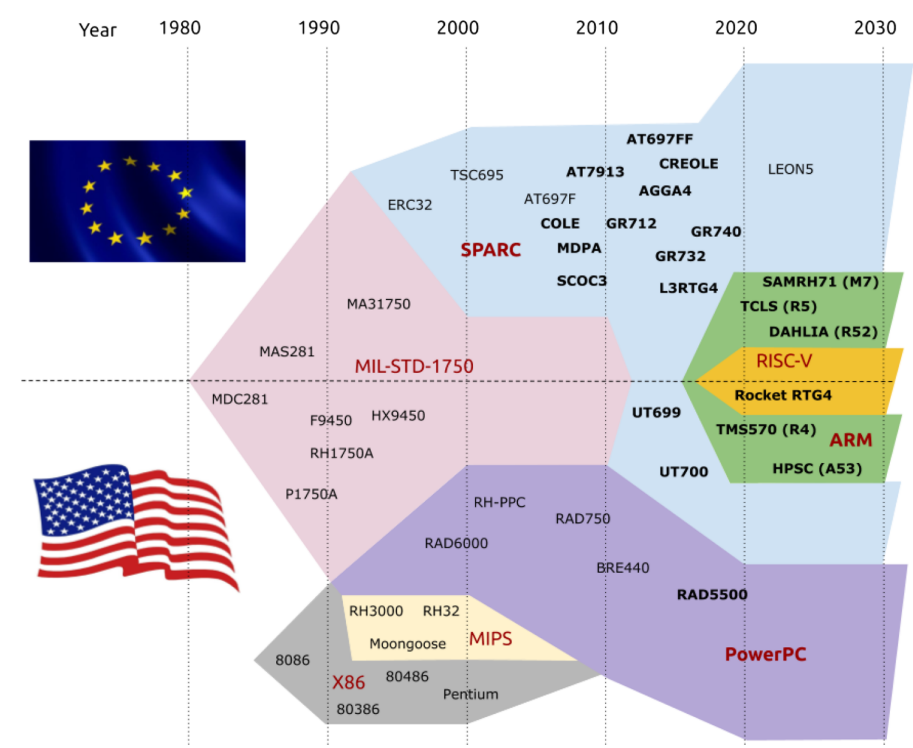
\includegraphics[width=0.6\linewidth]{Figures/CPUsHistory.png}
		\caption{History of CPU architectures used in space missions. Source: \cite{DiMascio2020}}
		\label{fig:CPU-Archs}
	\end{figure}
The European Space Agency (ESA) opted for the SPARC architecture, mainly because of the widespread availability of software and its open architecture, which allowed the Agency's independence from specific vendors. To this aim, ESA funded the development of the LEON processor in late 1997. One of the principal objectives of the project was the integration of fault tolerant-by-design techniques. The processor should be able to detect and tolerate one error in any register without software intervention, and to suppress effects from  Single Event Transient (SET) errors in combinational logic \cite{Anrersson2010}. LEON evolved in the following years and currently, LEON3 \cite{leon3} is the most widely adopted platform for ESA missions. LEON3 is distributed as synthesizable VHDL model of a 32-bit processor compliant with the IEEE-1754 (SPARC V8) architecture by Aeroflex Gaisler. The distribution is under the GNU GPL license allowing use for any purpose without licensing fee. The most significant upgrades over the previous LEON2 is the support of Symmetric Multi Processing (SMP) and pipelined operation at 5 stages. In space missions, a fault-tolerant version of the processor (LEON3FT) is the one that is widely used. Fault tolerance is assured by the implementation of ECC coding of all on-hip RAM blocks, which is able to detect and correct up to four errors per 32-bit RAM words or per cache memory tag, and all these without performance impact (completely transparent to user applications). The main means for achieving fault-tolerance is by using ECC coding of all on-chip RAM blocks. A famous LEON3-based SoC is the GR712RC from Aeroflex Gaisler.\par 
LEON5 is the latest version of  the LEON processor family\cite{leon5} and it primarily targets high-end FPGA's. Although it has not yet been implemented in space missions, it provides backward compatibility for most of the software implementations that have targeted LEON3 and LEON4 processors, claiming up to 85\% higher performance. Nevertheless, the Reduced Instruction Set Computer version V (RISC-V) Instruction Set Architecture (ISA) is expected to dominate upcoming on-board processing applications \cite{DiMascio2020}. In European missions for example, the De-RISC project \cite{derisc2020} has recently shown the first milestones for a multi-core RISC-V processor for aerospace designs. The project is based on the NOEL-V 64-bit RISC-V processor core \cite{noelv} from Aeroflex Gaisler and state-of-the-art hypervisor technology to accomplish high performance workloads, on a complete processing platform for space. The three processor models (LEON3/5, NOEL-V) are distributed as parts of the open-source GRLIB IP library, which is an integrated set of reusable IP cores, designed for system-on-chip (SoC) development and they are available also in fault-tolerant versions for FPGA and ASIC implementations. Typically, they are interconnected through Advanced Microcontroller Bus Architecture (AMBA) Advanced High-performance Bus (AHB) and Advanced Peripheral Bus (APB) interfaces. A typical SoC built around a single LEON/NOEL processor core with the peripherals included in the distribution is depicted in Fig. \ref{fig:LEONSoC}\par
	\begin{figure}
		\centering
		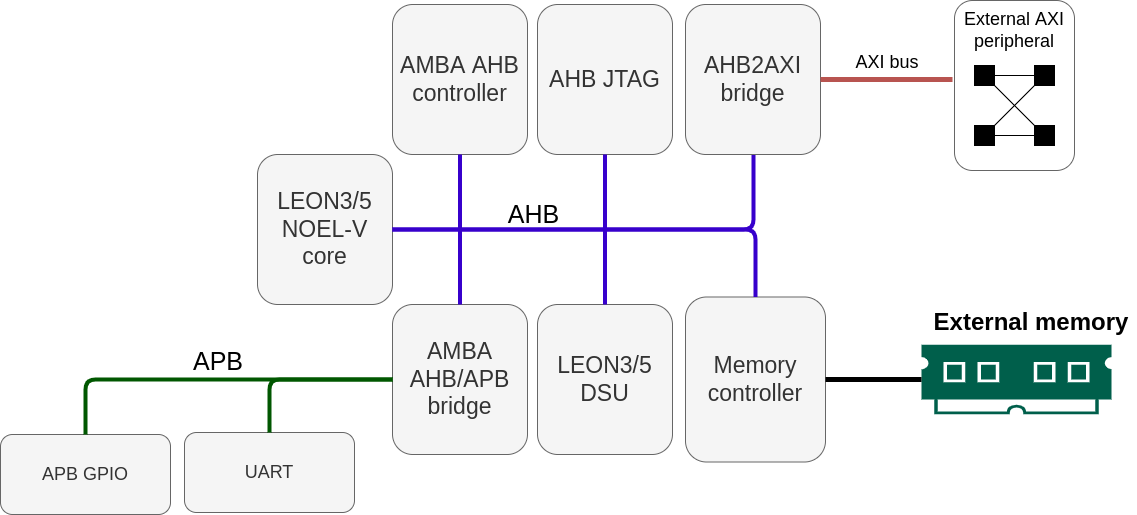
\includegraphics[width=0.8\linewidth]{Figures/LEONSoC.png}
		\caption{A typical LEON/NOEL SoC design}
		\label{fig:LEONSoC}
	\end{figure}
As its name implies, the AHB JTAG component shown in the image provides a JTAG debug link to the SoC, allowing among other things the uploading and debugging of user software to the processor's memory, through the GRMON software tool, which is part of the processor's software ecosystem. Other useful software tools included in the ecosystem are the cross-compiler for the CPU architecture and a simulator (TSIM). The debugging capabilities are completed with the Debug Support Unit (DSU) depicted in the image. This module communicates with the CPU through a dedicated debug interface (in addition to AHB) and has complete control over its pipeline, its registers and the contents of the instruction trace buffer. The processor can be set into debug mode by the DSU, which halts the pipeline. As part of the current work, the LEON/NOEL ecosystem has been set up on the KCU105 and Zedboard development board, to allow for interaction with custom FPGA peripherals, as well as for software comparison\par


\subsection{Spacewire and spacefibre}\label{subsubsec:spfi}
On-board processing systems examples are instruments, mass-memory, processors, and downlink telemetry. The interconnection of this systems is a challenging task:fault-tolerance, error recovery capabilities, low power, simplicity, performance and architectural flexibility place stringent requirements on the design of an on-board network. The interconnections of the equipment in such a network is feasible only with serial links. \cite{Athavale2005}.\par
Initially, space agencies and manufacturers followed their proprietary approaches to address this issue. The diversity of communication links that arose resulted in high cost, limited development and test time and interoperability issues. In 1992, the demand for interconnection of distributed signal-processing systems led ESA to assign the development of a new standard to the University of Dundee \cite{Parkes2012}. This process resulted in the first version of ECSS-E-ST-50-12C (SpaceWire) standard \cite{spwire}.
The standard defined a high speed data-handling on-board network and technology. It provides bidirectional, full-duplex data-links at speeds of 2 Mbit/s to 200 Mbit/s, which connect together SpaceWire enabled equipment. Data-handling networks can be built to suit particular applications using point-to-point data-links and routing switches.\par
	\begin{figure}
		\centering
		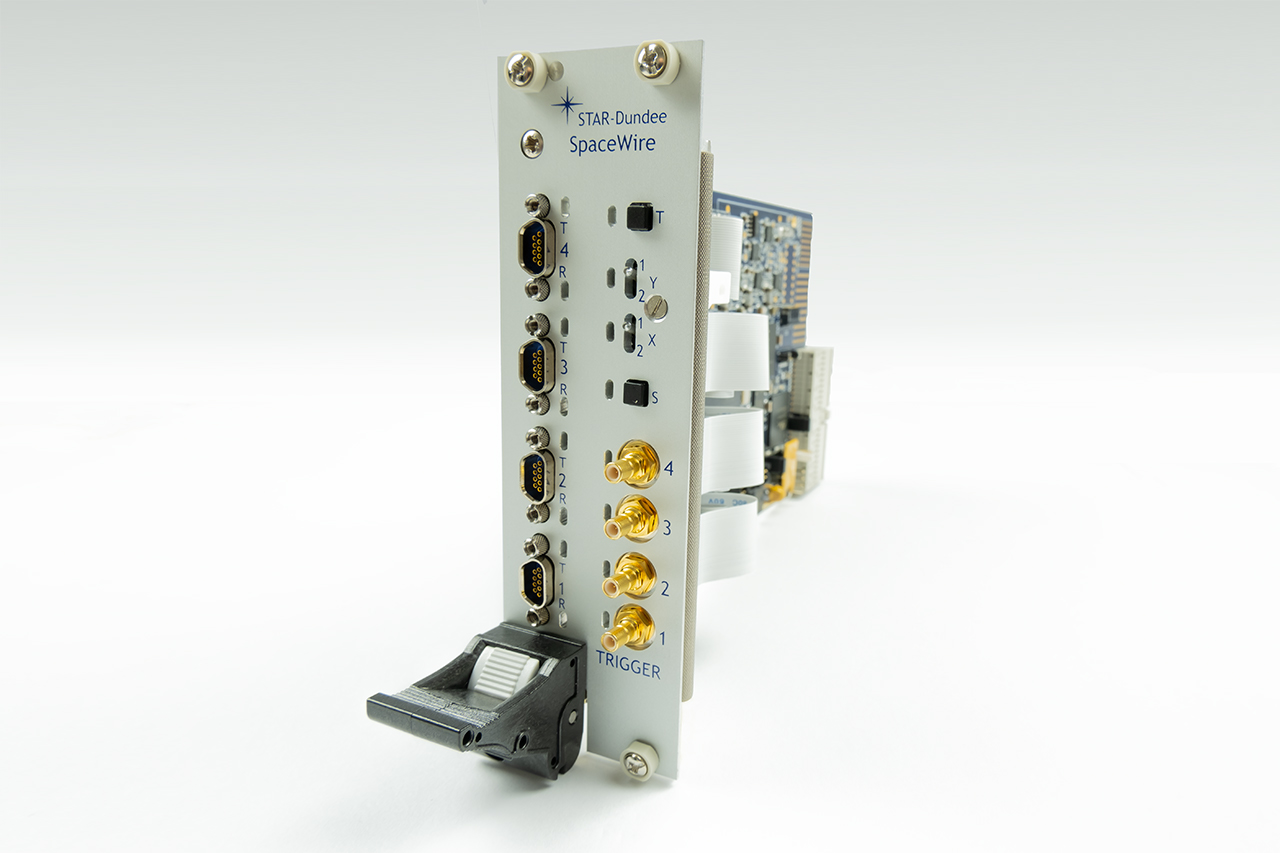
\includegraphics[width=0.6\linewidth]{Figures/pxi_interface_8hp_front.jpg}
		\caption{SpaceWire PXI Mk2 card from STAR-Dundee. (source: https://www.star-dundee.com/products/spacewire-pxi-mk2/)}
		\label{fig:A}
	\end{figure}
The next generation of SpaceWire is the SpaceFibre technology, standardised as ECSS-E-ST-50-11C \cite{spfibre}. Except for higher data rates (6,25 Gbps signalling rated), SpaceFibre comes with other significant enhancements:
\begin{itemize}
    \item Fibre-optic cabling, with electrical support for backwards compatibility with SpaceWire.
    \item Multi-laning, which can combine the throughput of multiple physical links (lanes) to support well over 20 Gbit/s.
    \item Advanced Quality of Service (QoS) mechanisms, like prioritization of Virtual Channels, bandwidth reservation and support of deterministic delivery constraints.
\end{itemize}
DSCAL is a partner of the Hi-SIDE project (https://www.hi-side.space/) consortium and as such, it has been granted a access to SpaceFibre test equipment, featuring a STAR-Ultra PCIe interface and link analyzer card (https://www.star-dundee.com/products/star-ultra-pcie), along with the necessary software tools (GUI and API for the development of custom applications and performance measurements). An accompanying encrypted IP core netlist, adds transparency in the communication of the software channel interface on the host PC's application with the logic implemented on an FPGA. The core exposes up to 7 AXI4-Stream 128-bit interfaces to the user logic and a RMAP port for configuration and control.\par
The provided equipment can provide two 4-lane SpaceFibre links to a suitable corresponding interface of up to 20 Gbit/s per link, depending on the number of SFP interfaces of the available FPGA platforms. The maximum data rate can be achieved when all four 6,25 Gbit/s lanes are used. Because of the 8b/10b encoding on the SpaceFibre link, only 80\% of the lane bandwidth is available to the user logic. Of the equipment available at DSCAL, only the Zynq UltraScale+ MPSoC ZCU102 development board with 4 SFP+ connector cases can support the maximum data rate of 20 Gbit/s. The ZCU105 card, however, which has been extensively used in this work can only provide up to 10 Gbit/s of user bandwidth.\par
	\begin{figure}
		\centering
		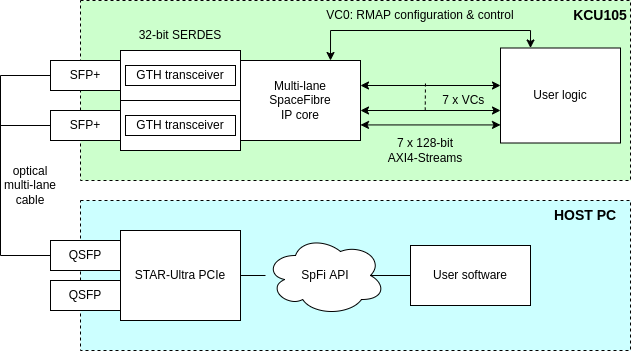
\includegraphics[width=0.6\linewidth]{Figures/SpFibre.png}
		\caption{Block diagram of the SpaceFibre equipment and environment}
		\label{fig:equipment}
	\end{figure}
As part of the Hi-Side project's deliverables, a sample design for the KCU105 had been provided to DSCAL. The reference design included a basic demo for a loopback test through the card's FMC connectors, without connectivity to the host PC. The reference design had to be modified, so that SERDES is mapped to the transceivers allocated to the SFP+ connectors of the board. The transceivers needed also to be parametrized and a suitable clock source to be configured on the board and connected to the transceivers' CPLLs. This process was different for the equipment used in DSCAL: the KCU105 and ZCU102 boards use GTH transceivers, while ZC706 uses GTX transceivers. Figure \ref{fig:equipment} is a block diagram of the resulting environment used for testing. The design depicted refers to the configuration used on the KCU105 board, but except for the number of lanes and type of transceivers, it is the same for all the other boards.\par
	\begin{figure}
		\centering
		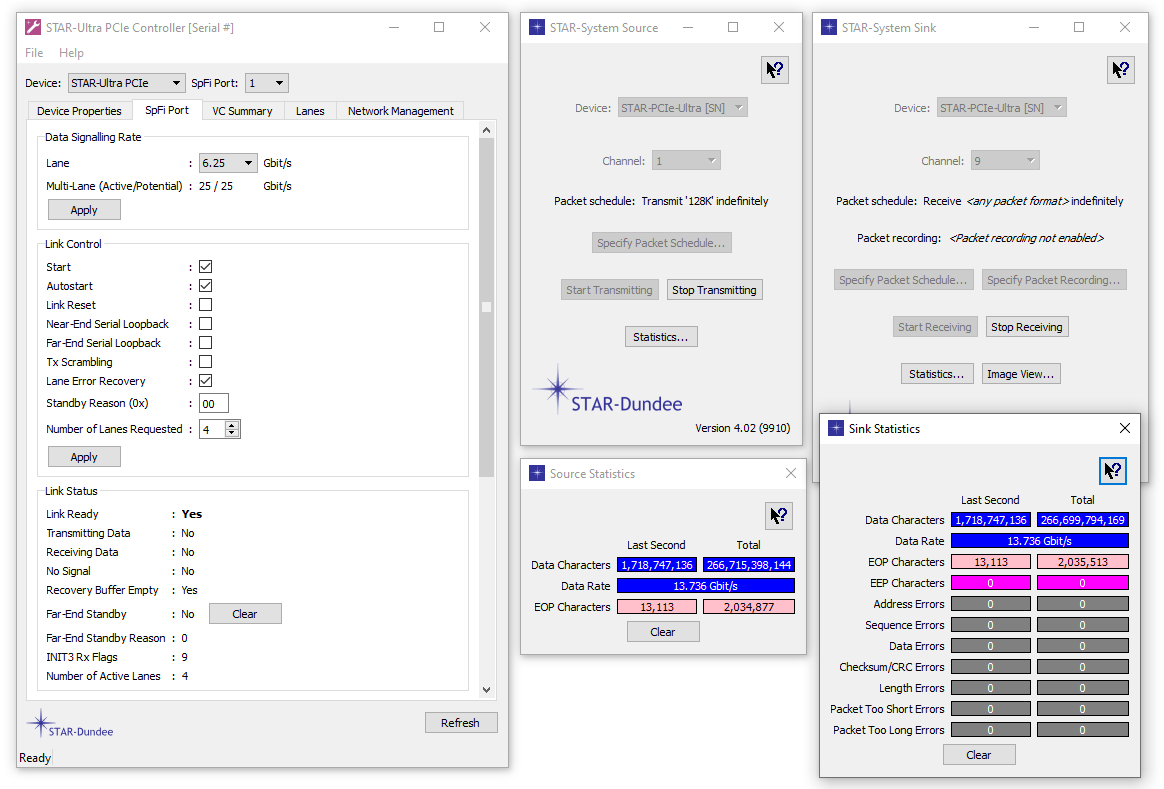
\includegraphics[width=0.6\linewidth]{Figures/star-ultra_pcie_tx_and_rx.png}
		\caption{GUI applications examples}
		\label{fig:gui}
	\end{figure}
On the PC side, the STAR-System software provided as part of the Hi-SIDE equipment provides the drivers of the SpaceFibre STAR-Ultra PCIe board, as well as the software tools for transmitting and receiving packets to and from the SpaceFibre IP code. The software bundle provides two options: a set of GUI applications and a complete API for the development of custom software tools. In both cases, statistics and performance data can be derived. Figure \ref{fig:gui} gives an example of the GUI applications. In order to streamline the automatic execution of scripts including SpaceFibre transactions, the following custom applications were developed, based on the STAR-System API:
\begin{itemize}
    \item rmapRead $<address>$: reads a 4-byte register at a user-specified address.
    \item rmapWrite $<address> <value>$: writes a 32-bit value at a register at a user-specified address.
    \item sendFile -c $<channel> -i <file>$: sends a binary file to the specified channel of the master stream interface of the core.
    \item sendFile -c $<channel> -i <file>$: receives data from the specified channel until an End Of Packet (EOP) character is sent and writes the stream into a file.
\end{itemize}

\subsection{Bit-level channel coding}
partial recofiguration on xupv5
testing with matlab model
\subsection{Magnetic recording media coding}
\subsection{Packet-level coding}
Do not forget to add the memory subsystem we created for LEON on ZynQ system (access to DDR memory through
